\documentclass[../main.tex]{subfiles}
\graphicspath{{\subfix{../images/}}, {\subfix{../}}}

\begin{document}

\chapter{EG-X model}

\epigraph{Test}{Test source}

The tight-binding Hamiltonian for the model reads
\begin{align}
	H_0 = &-t_{\mathrm{X}} \sum_{\langle ij \rangle, \sigma} d_{i, \sigma}^{\dagger} d_{j, \sigma}
	-t_{\mathrm{Gr}} \sum_{\langle ij \rangle, \sigma} \left(
	c_{i, \sigma}^{(A), \dagger} c_{j, \sigma}^{(B)} +
	c_{j, \sigma^{\prime}}^{(B), \dagger} c_{i, \sigma}^{(A)} \right) \notag \\
	&+ V \sum_{i, \sigma} d_{i, \sigma}^{\dagger} c_{i, \sigma}^{(A)} + \mathrm{h.c.} \label{eq:EG-X model Hamiltonian non-interacting}
\end{align}
with:
\begin{itemize}
	\item \(d\) operators on the \(\mathrm{X}\) atom
	\item \(c^{(\epsilon)}\) operators on the Graphene site (\(\epsilon = A, B\))
	\item \(t_X\) next-nearest hopping for the \(\mathrm{X}\) atoms
	\item \(t_{Gr}\) next-nearest hopping on the Graphene
	\item \(V\) hopping between \(\mathrm{X}\) and Graphene \(\mathrm{B}\) sites
\end{itemize}
This describes the

\begin{figure}[t]
	\begin{subfigure}{0.5\linewidth}
		\centering
		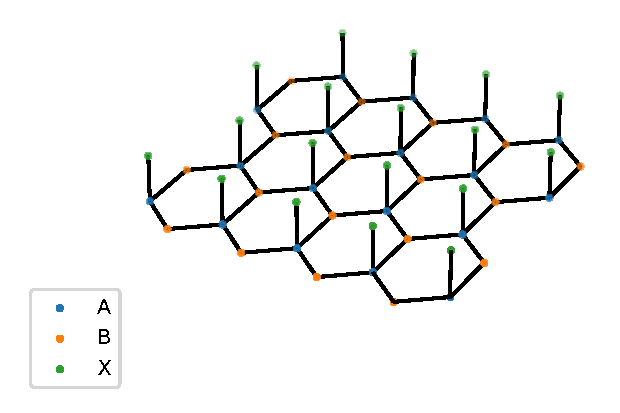
\includegraphics[width=\linewidth]{images/eg-x lattice cropped}
		\caption{EG-X model}
		\label{fig:eg-x model}
	\end{subfigure}
	\begin{subfigure}{0.5\linewidth}
		\centering
		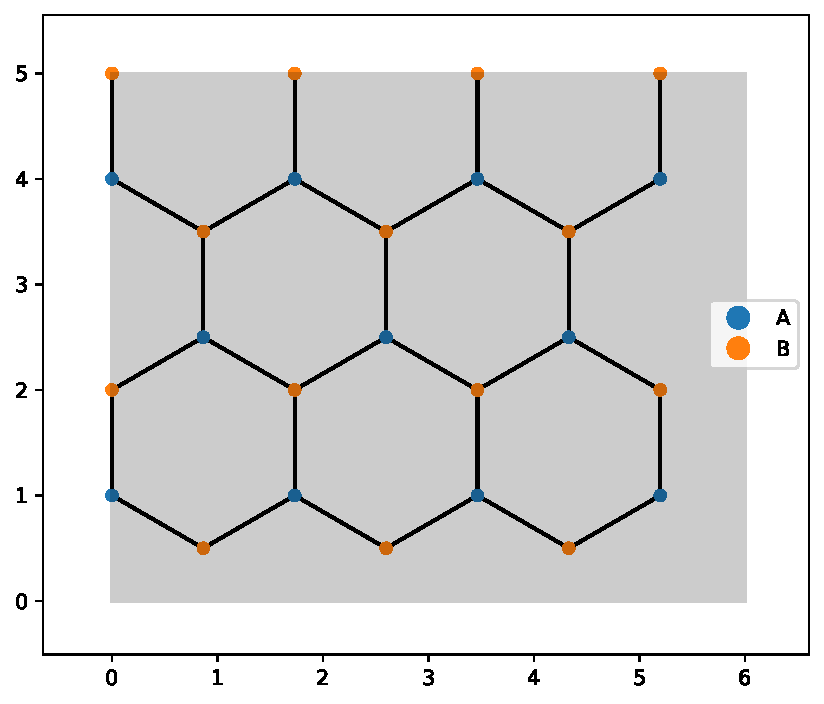
\includegraphics[width=\linewidth]{images/graphene lattice}
		\caption{Graphene lattice structure}
		\label{fig:graphene lattice structure}
	\end{subfigure}
\end{figure}
In material terms, this can be thought of as a sheet of graphene on top of another material, providing the additional \(\mathrm{X}\) atoms, but in this thesis the model will be taken as a toy model, providing certain favorable aspects.


\section{Lattice Structure of Graphene}\label{sec:lattice-structure-of-graphene}

This section reviews the lattice structure of graphene and by extension also of the flat-band model, following the review~\cite{yangStructureGrapheneIts2018}.

Monolayer graphene forms a hexagonal lattice as seen in \cref{fig:graphene lattice structure}.
This is formed by two triangular sub lattices, so the unit cell of the hexagonal lattice has two atoms.
The primitive vectors of the hexagonal lattice are
\begin{align}
	\vb{a}_1 &= \frac{a}{2} \begin{pmatrix} 1 \\ \sqrt{3} \end{pmatrix} \notag\\
	\vb{a}_2 &= \frac{a}{2} \begin{pmatrix} 1 \\ -\sqrt{3} \end{pmatrix}
	\;,
\end{align}
with lattice constant \(a \approx \qty{2.46}{\angstrom}\) for graphene.
The distance between nearest neighbor is
\begin{equation}
	a = \sqrt{3} a_0 \;.
\end{equation}

The primitive reciprocal lattice vectors \(\vb{b}_1\), \(\vb{b}_2\) fulfill
\begin{align}
	\vb{a}_1 \cdot \vb{b}_1 &= \vb{a}_2 \cdot \vb{b}_2 = 2\pi \notag\\
	\vb{a}_1 \cdot \vb{b}_2 &= \vb{a}_2 \cdot \vb{b}_1 = 0
	\;,
\end{align}
so
\begin{align}
	\vb{b}_1 &= \frac{2\pi}{a} \begin{pmatrix} 1 \\ \frac{1}{\sqrt{3}} \end{pmatrix} \notag\\
	\vb{b}_2 &= \frac{2\pi}{a} \begin{pmatrix} 1 \\ - \frac{1}{\sqrt{3}} \end{pmatrix}
	\;.
\end{align}
\todo{Graphic for primitive BZ}
\todo{Explain primitive BZ}
\todo{Explain: what symmetries does EG-X break? How does that influence BZ?}

Points of high symmetry in the Brillouin zone are:
\begin{align}
	\Gamma &= \begin{pmatrix} 0 \\ 0 \end{pmatrix} \\
	\mathrm{M} &= \frac{\pi}{a} \begin{pmatrix} 1 \\ \frac{1}{\sqrt{3}} \end{pmatrix} \\
	\mathrm{K} &= \frac{4\pi}{3 a} \begin{pmatrix} 1 \\ 0 \end{pmatrix}
	\;.
\end{align}

\begin{figure}[t]
	\centering
	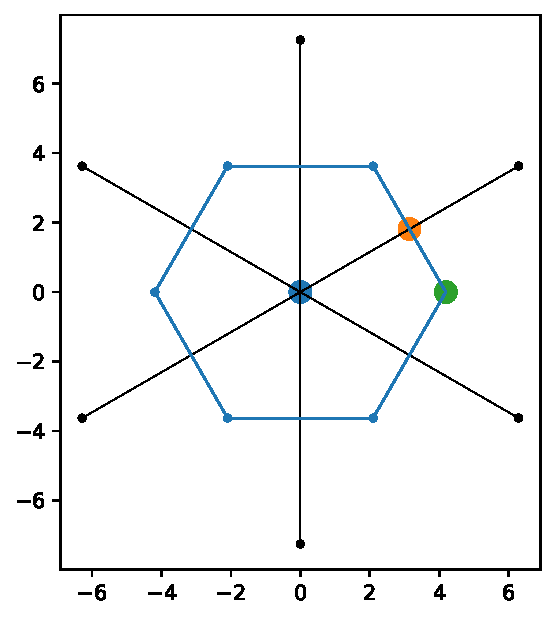
\includegraphics[width=0.5\textwidth]{images/graphene brillouin_zone}
	\caption{Graphene Brillouin Zone}
	\label{fig:graphene Brillouin zone}
\end{figure}

\section{Band structure}

aka why is the model interesting?

The detailed derivation can be found in \cref{ch:EG-X Hamiltonian in Reciprocal Space}.

\begin{align}
	H_0 &= \sum_{\vb{k}, \sigma} \begin{pmatrix} c_{k, \sigma}^{A, \dagger} & c_{k, \sigma}^{B, \dagger} & d_{k, \sigma}^{\dagger} \end{pmatrix}
	\begin{pmatrix}
		0 & f_{Gr} & V \\
		f_{Gr}^* & 0 & 0 \\
		V & 0 & f_{X}
	\end{pmatrix} \begin{pmatrix} c_{k, \sigma}^{A} \\ c_{k, \sigma}^{B} \\ d_{k, \sigma} \end{pmatrix}
	\label{eq:EG-X Hamiltonian non-interacting matrix}
\end{align}
	
	
\end{document}